% PREAMBULO
\documentclass[10pt, a4paper]{article}
	% Tamaño de letra, clase de documento, y otros estilos. Necesario para definir el documento

% PAQUETES
\usepackage{geometry}
%\usepackage[spanish]{babel}
\usepackage{amsmath}
\usepackage[utf8]{inputenx}
\usepackage{fancyhdr}
%\usepackage{breakurl}
\usepackage{graphicx}
%\usepackage{multicol}
\usepackage[unicode=true, bookmarks=true,bookmarksnumbered=false,bookmarksopen=false, breaklinks=false,pdfborder={0 0 0},backref=false,colorlinks=true,linkcolor=blue,urlcolor=blue,citecolor=blue] {hyperref}
\usepackage{colortbl}
%\usepackage{hyperref}
%\usepackage{helvet}


% GEOMETRÍA
	% Derivada del paquete geometry. Definimos la geometría del documento -los márgenes-
\geometry{verbose,lmargin=30mm,rmargin=30mm}


% FUENTES
	% Se activa que la fuente por defecto sea 'sans serif'
%\renewcommand{\familydefault}{\sfdefault}


% HEADINS & FOOTERS
	% Configuran el paquete fancyhdr
\setlength{\headheight}{10pt}
%\pagestyle{fancyplain}
\pagestyle{fancy}
\fancyhf{}
\lhead{\footnotesize DIGITAL IMAGE PROCESSING}
\rhead{\footnotesize OPTICAL MUSIC RECOGNITION \thepage}
\rfoot{\footnotesize UNIVERSIDAD DE GRANADA}
\lfoot{\footnotesize TELECOMMUNICATIONS ENGINEERING}


% CONFIGURAR ESTOS PARAMETROS
\hypersetup{
  pdftitle={Optical Music Recognition},
  pdfauthor={Antonio Moya y Fernando Pérez},
  pdfsubject={Procesamiento Digital de Imágenes},
  pdfkeywords={Reconocedor}{Óptico}{Partituras}{UGR}{Proyecto}}


% TITULO DEL DOCUMENTO
\title{\textsc{Optical Music Recognition}}
\author{Antonio José Moya Díaz \and Fernando Pérez Bueno}
\date{}


\begin{document}
\maketitle

ABSTRACT.- This document presents the steps and the decisions taken in the implementation of this project of optical music recognition. There are three main steps. Firstly, every element needs to be isolated. Then the element is recognized to identify which element is. Finally, in case of being a note, the value is calculated depending on its position on the score.


\section{Introduction}

The work presented in this document was the final project for the course \emph{Digital Image Processing}. The aim of this project was to learn and train certain skills in the field of image processing instead of creating a complete music recognition software. That is why this project presents several limitations. 

In the following sections the whole process is explained in detail, these limitations are pointed out and, in most cases, solutions for these limitations are given for possible future versions of this project.


\section{Segmentation}

It is essential for reading the score to focus on each of its elements one by one. Each element needs to be isolated in a single image in order to proceed with its identification.

The first step to achieve this is to divide the image horizontally using the function \emph{corte\_horizontal}. Thus, every horizontal element will be divided in a separate image (figure \ref{fig1}). These elements will be the staff and also every add-on that the image may contain such us title, author, lyrics, etc.

\begin{figure}[h!]
  \centering
    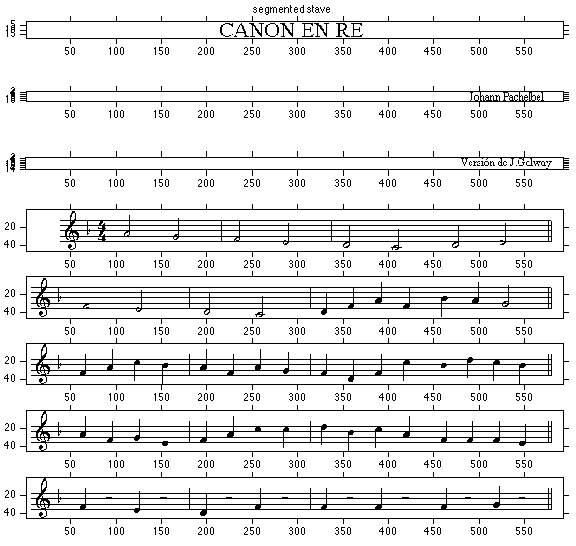
\includegraphics[scale=0.3]{./img/img1.png}
  \caption{Output of the function corte horizontal}
  \label{fig1}
\end{figure}

Then, the function \emph{recon\_pentagramas} is applied to the images obtained in the previous step. This function saves the images which contain staves while dismissing the other images. Staves are identified calculating histograms for every image and selecting those ones which have a stave-like histogram. Those histograms contain five maximums, one for each line of the stave.

\begin{figure}[h!]
  \centering
    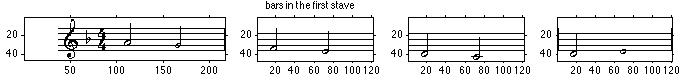
\includegraphics[scale=0.5]{./img/img2.png}
  \caption{Output of the function separar compases}
  \label{fig2}
\end{figure}


The second step is to divide the staves into bars. This task is easy given that each bar-line presents a maximum in a vertical histogram of every single stave. However, some staves do not have a bar-line at the beginning neither at the end, so the requirements to divide need to be relaxed and then filter the divided segments to recognize which ones are bars. This process is made by the function \emph{separar\_compases} (figure \ref{fig2}).

The final step of the segmentation process is to isolate any element inside every bar. This is made by the function \emph{separar\_elementos} which uses histograms again (figure \ref{fig3}). 

\begin{figure}[h!]
  \centering
    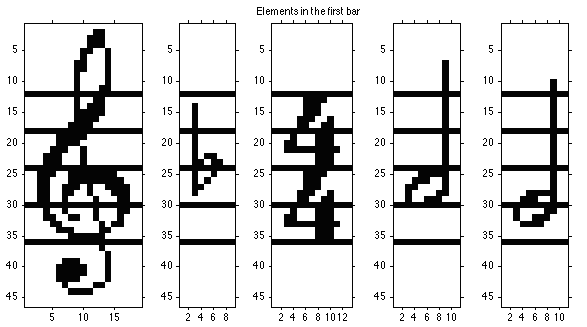
\includegraphics[scale=0.25]{./img/img3.png}
  \caption{Output of the function separar elementos}
  \label{fig3}
\end{figure}

The bar splitting is not truly needed given that this software can detect every element directly. However, this bar segmentation throws data which could be used in future or complex versions of this project.

\section{Element Identification}

At this point every element found in the stave is in a separate image. The next step is to identify which element is. However, before the identification, the image needs to be cleaned up in order to erase the stave lines. Finally the image is compared through correlation with the elements stored in the database. This way name and type of the element will be determined according to the elements in the database.

\begin{figure}[h!]
  \centering
    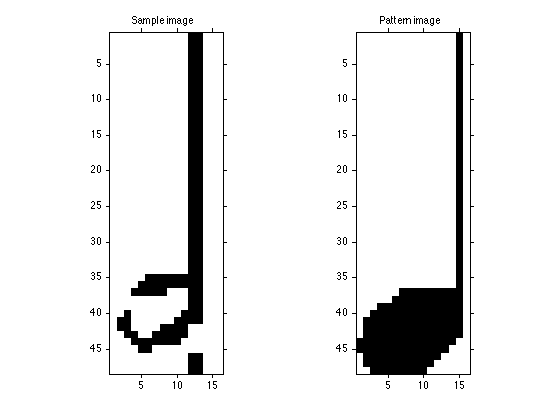
\includegraphics[scale=0.15]{./img/img4.png}
  \caption{Comparison between the sample image to recognize (left) and a pattern image (right)}
  \label{fig4}
\end{figure}

\subsection*{Database}

The database used in this project is a very basic one, which contains only the elements needed to identify the scores given. Nevertheless, it was done in a scaleable way so the addition of new elements is easy. The database is organized in 3 tables: one for notes, one for rests and one for other elements. 

\begin{figure}[h!]
  \centering
    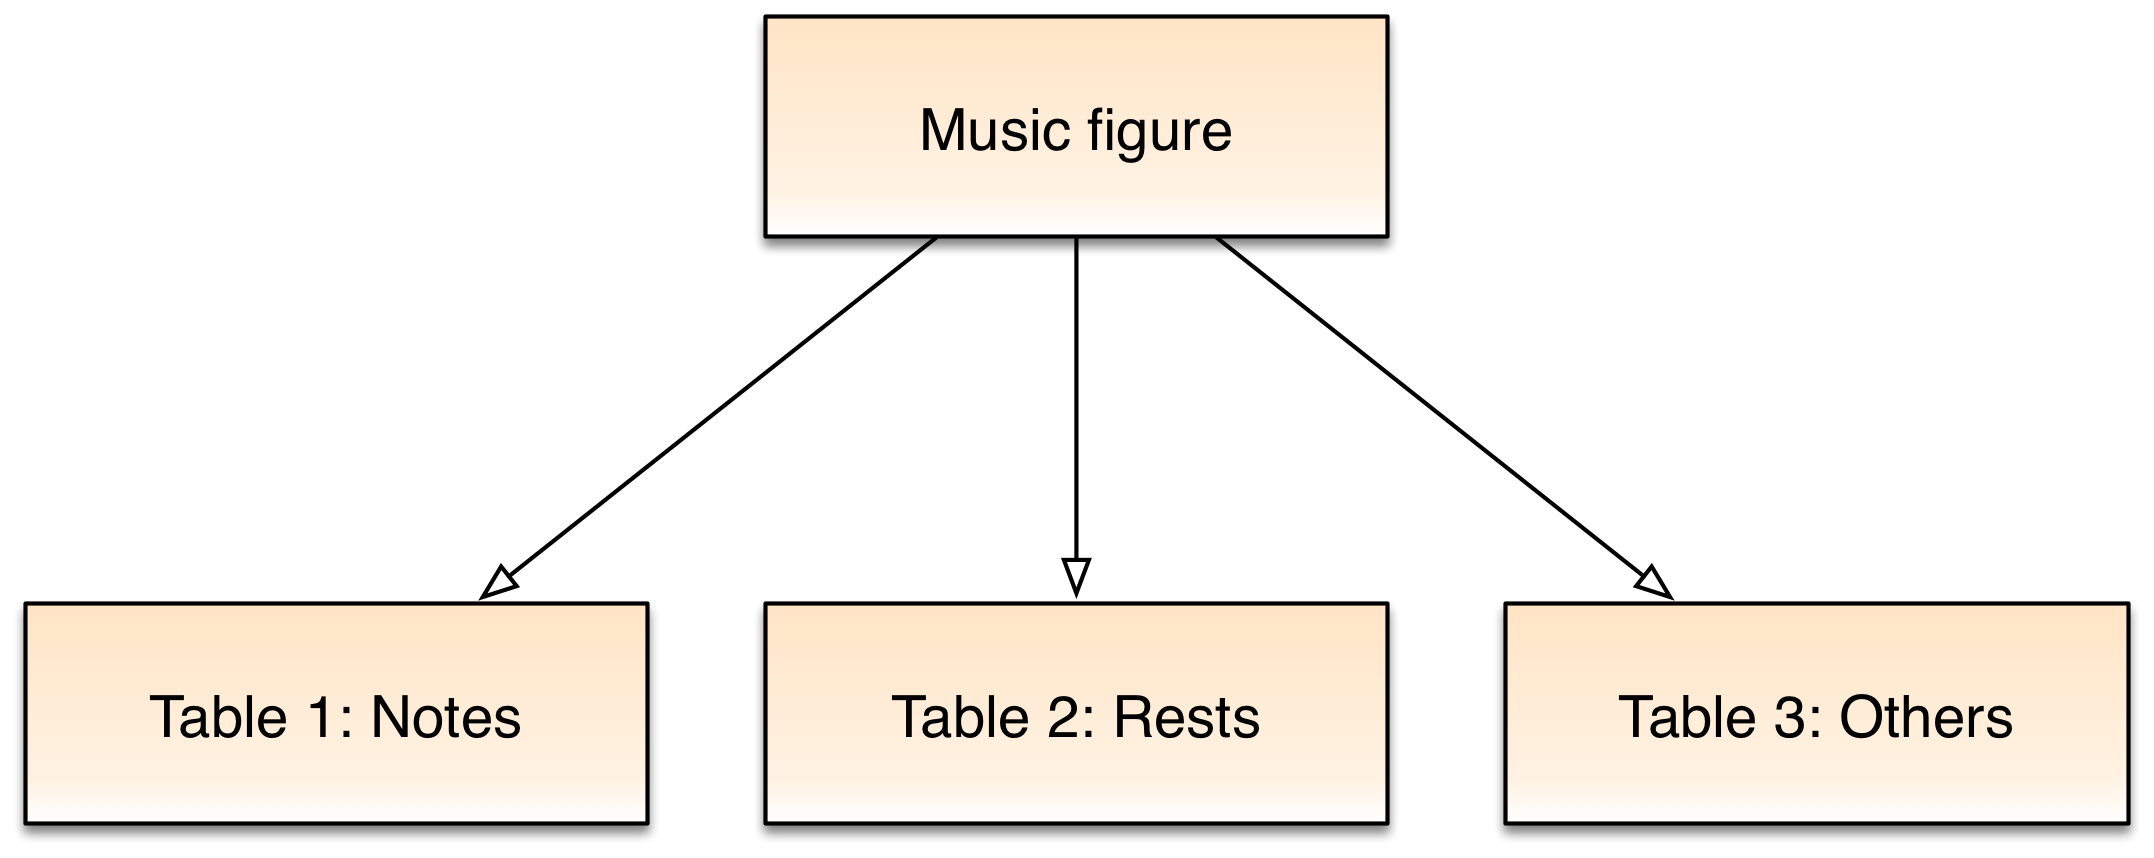
\includegraphics[scale=0.4]{./img/BD.png}
  \caption{Database hierarchy}
  \label{figBD}
\end{figure}

In case of identifying a note, the information of its pitch needs to be calculated. In case of a rest, only the information of its time length is needed. In contrast, this software does not calculate the information of the elements in the third group (clefs, time signatures, etc) but, as the element is recognized, this information could be obtain in a future version of this project.

Besides the organization of the database, it is important to use pattern images properly selected to match with the elements to be identified. If the element is not correctly centered in the pattern image or it is not correctly sized the success rate of the comparison will decrease significantly.

\section{Pitch}

After recognize a note, it is necessary to determine its pitch.  Using the horizontal histogram, the note head is isolated.

\begin{figure}[h!]
  \centering
    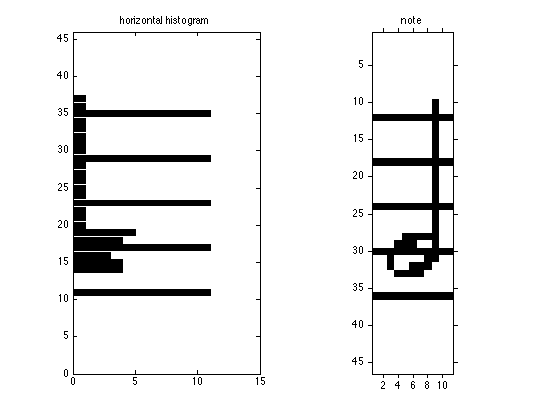
\includegraphics[scale=0.35]{./img/img5.png}
  \caption{Note and its horizontal histogram}
  \label{fig5}
\end{figure}

Then the image is divided in as many horizontal areas as pitches can be measured. These areas are calculated dynamically according to the stave, its size, and the space between the lines. The pitch is calculated just checking in which area the note head is.

\begin{figure}[h!]
  \centering
    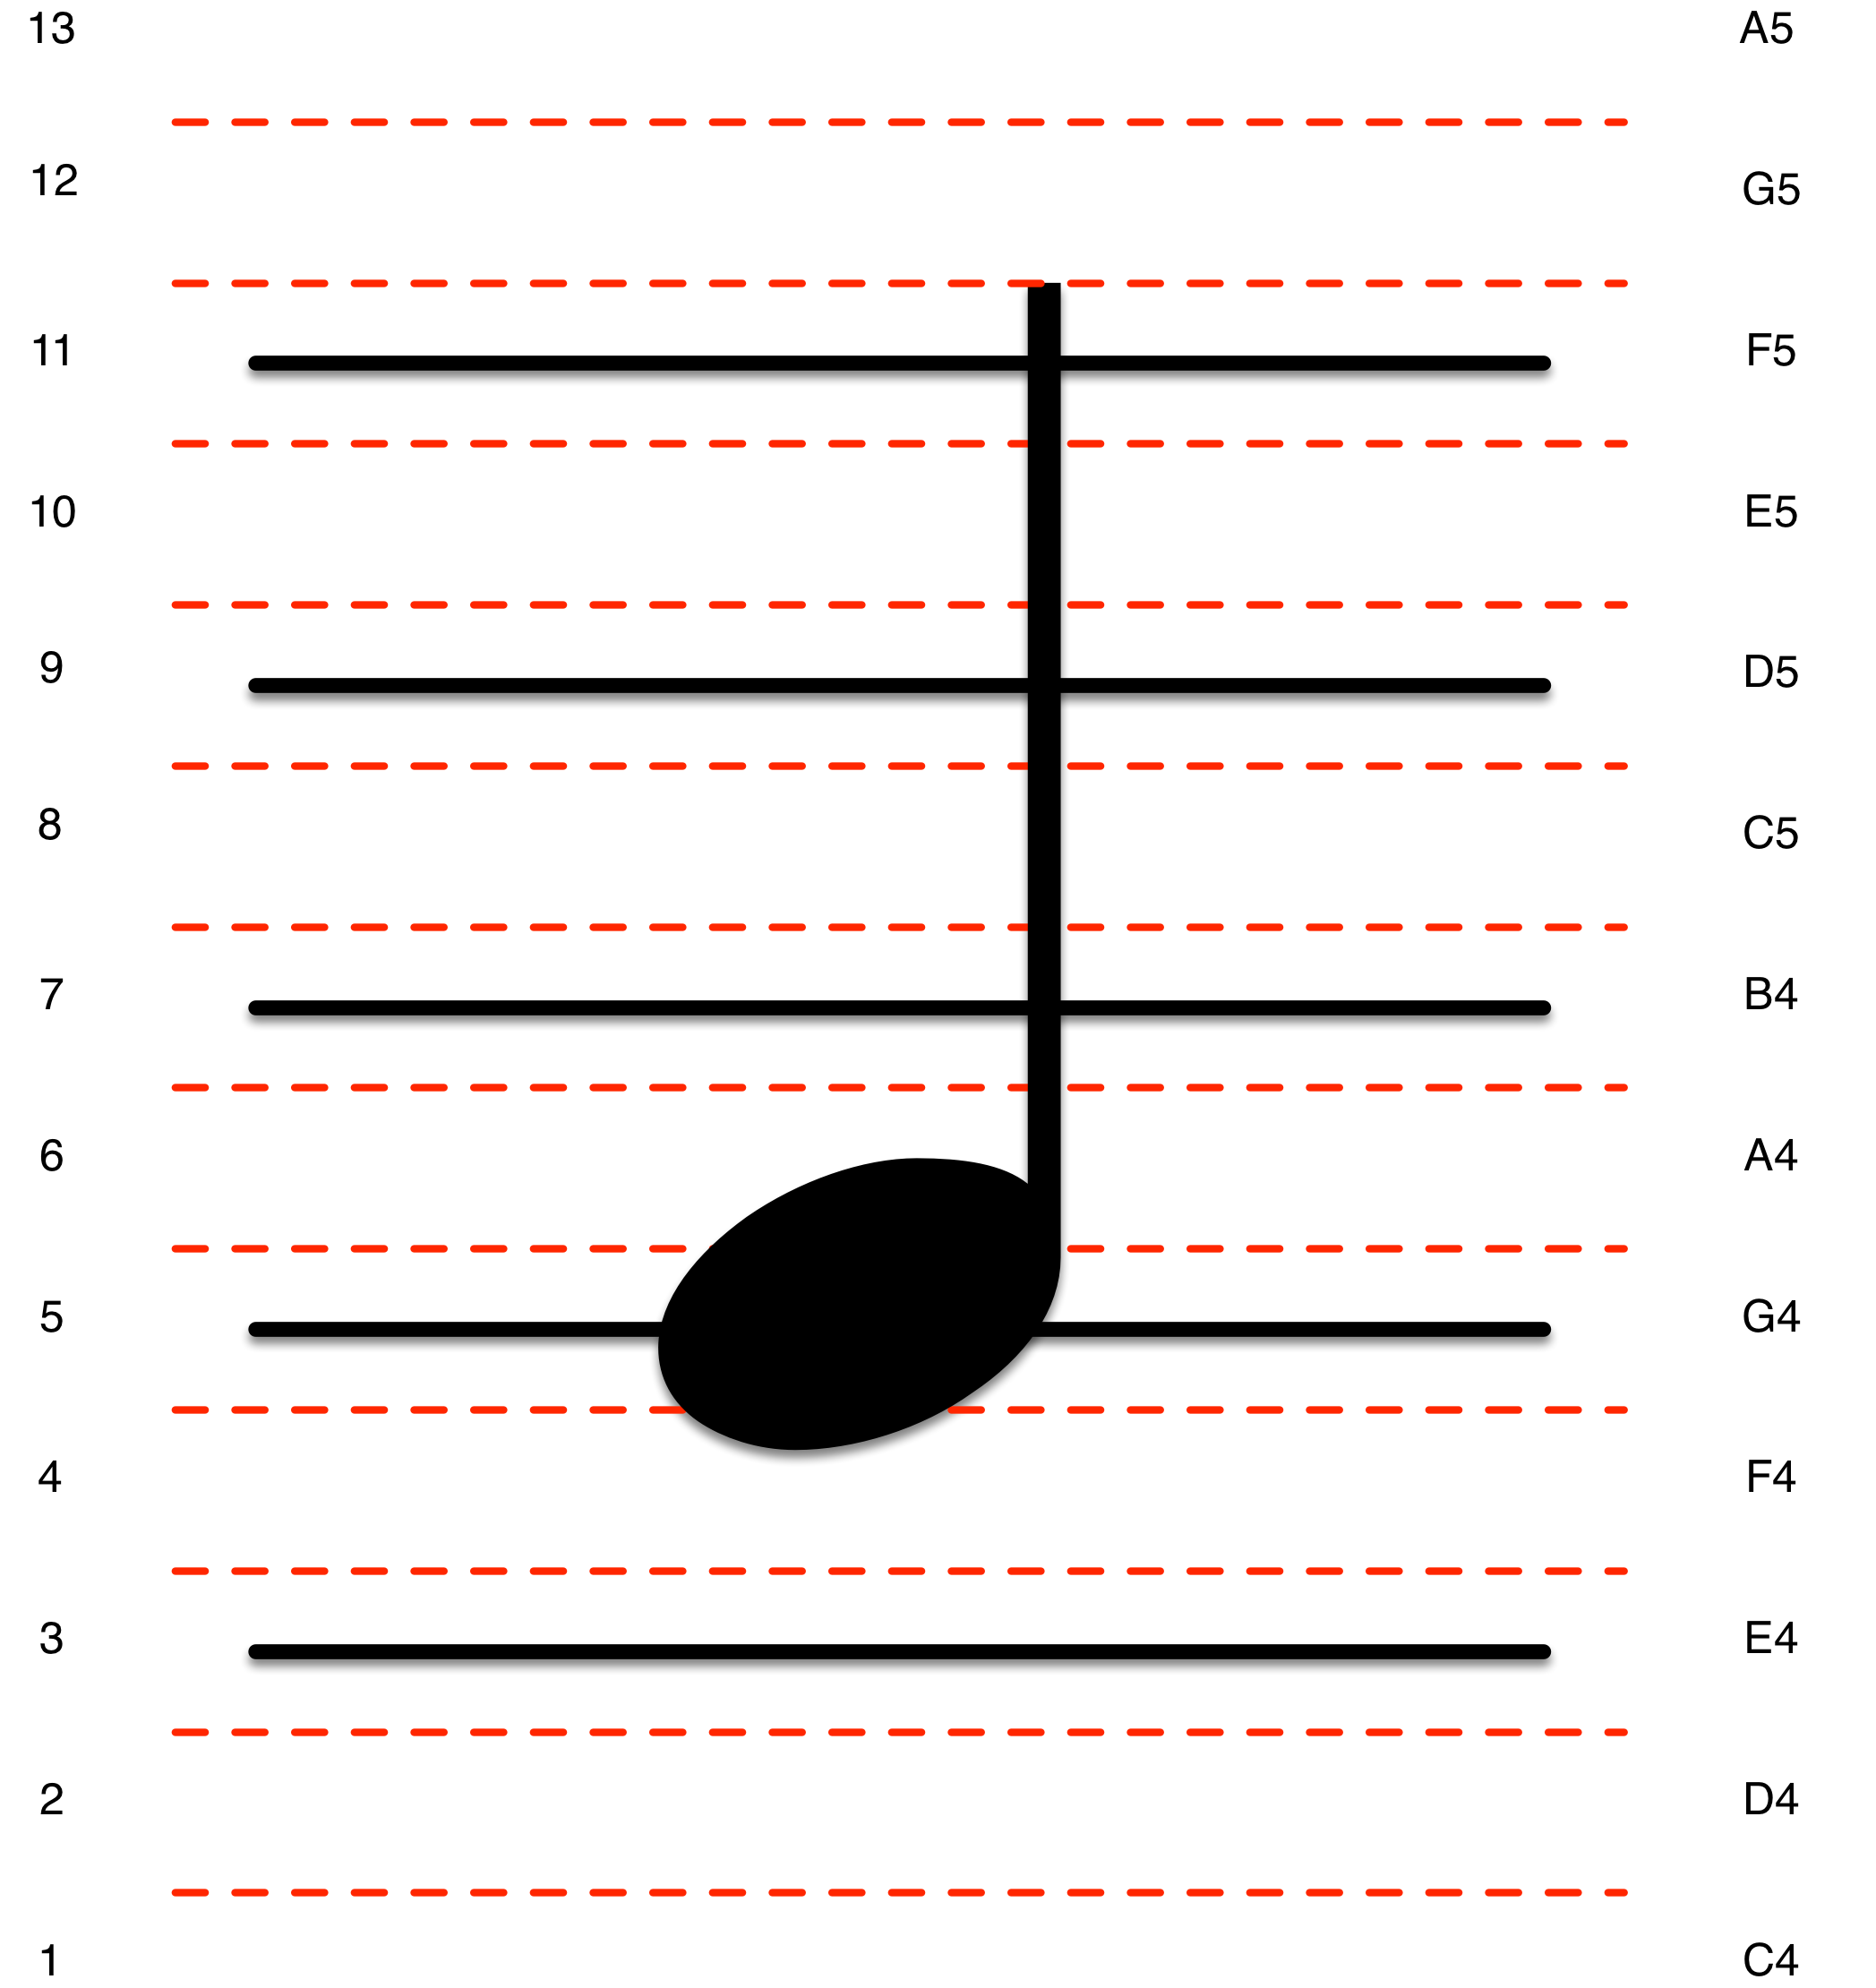
\includegraphics[scale=0.4]{./img/pitch_spaces.png}
  \caption{Space division scheme}
  \label{fig_pitch}
\end{figure}

Note that each position in the stave represents a pitch, but what pitch is depends on the Clef. This project calculates pitches considering it is always the G-Clef. However, this software is capable of recognizing the Clef so it would be easy,  for future versions, to make the pitch calculation clef-sensitive.

The implemented procedure works only with simple notes, but it can be extended to recognize chords (more than one note at the same time). This could be done by checking the length of the head note positions (in case of two head notes were too close) or if more than one head note were detected (in case of two separated head notes).

\section{Process}

To sum up, for reading the score the first step is to isolate the staves, then the bars in the stave and, finally, every element in each bar. Then, after finishing  stave, the software follows up with the next stave and so on up to finish the score. 

Information extracted from each element is stored in a string variable in which newline is added after every stave in order to make a clearer display.

\section{Conclusions}

Although this is not a conceptually complex project, several problems were found during its development. Most of the notes are similar in shape, so the cleaning process needs to be very precise in order to correctly identify the image. In particular, whole and half rests are so similar that an extra checking was needed.


A fairly good quality pattern images were also needed. In fact, it seems that reduction in the size of the image to be identified decreases highly the success rate so that it is needed that the pattern image will always be bigger than the sample image.

Moreover, the development process should be done in the most generic way because trying to improve the recognition of a specific note value can damage others.\\ 

All these problems shows that the use this pattern recognition process alone is bit poor, and the whole process should be improve by using other techniques, for example, statistics based methods.


\end{document}